% 93-27(93쪽) — ∠C 의 이등분선 CD 를 그은 삼각형 ABC(원문 「오른쪽 그림」). 스캔 화질이 낮아 TikZ 로 다시 그림.
% 라벨은 원문 것만: 꼭짓점 A·B·C·D, 길이 6·3·2, 이등분을 나타내는 두 점 표시. 선분 AB 의 길이(답)는 그림에 적지 않는다.
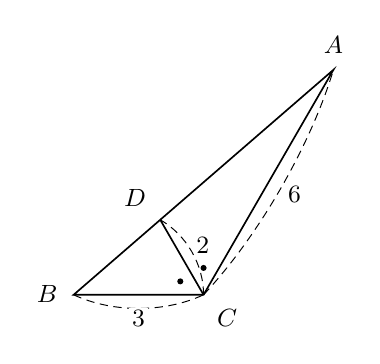
\begin{tikzpicture}[line width=0.6pt, x=0.55cm, y=0.55cm]
  \coordinate (A) at (6,5.196);
  \coordinate (B) at (0,0);
  \coordinate (C) at (3,0);
  \coordinate (D) at (2,1.732);
  \draw (A) -- (B) -- (C) -- cycle;
  \draw (C) -- (D);
  % 두 각이 같음을 나타내는 점 표시(원문)
  \fill (2.463,0.310) circle (1.1pt);
  \fill (3.000,0.620) circle (1.1pt);
  % 길이 표시의 점선 호
  \draw[densely dashed, line width=0.35pt] (C) .. controls (4.264,1.349) and (5.464,3.427) .. (A);
  \draw[densely dashed, line width=0.35pt] (B) .. controls (0.90,-0.42) and (2.10,-0.42) .. (C);
  \draw[densely dashed, line width=0.35pt] (C) .. controls (3.003,0.695) and (2.603,1.387) .. (D);
  \node[font=\small, anchor=south] at (6.00,5.33) {$\pt{A}$};
  \node[font=\small, anchor=east] at (-0.14,0.02) {$\pt{B}$};
  \node[font=\small, anchor=north west] at (3.08,-0.10) {$\pt{C}$};
  \node[font=\small, anchor=south east] at (1.90,1.80) {$\pt{D}$};
  \node[font=\small] at (5.10,2.32) {$6$};
  \node[font=\small, fill=white, inner sep=1pt] at (1.50,-0.55) {$3$};
  \node[font=\small, fill=white, inner sep=1pt] at (2.98,1.14) {$2$};
\end{tikzpicture}
